% ======================================================================
%  Chapter 14 — One Dimension  (EXPANDED)
% ======================================================================

\section{Topology in one dimension}
\label{sec:ch14-1d-topology}

One-dimensional systems are the simplest arena in which topological
ideas appear.  There is no Chern number in 1D---the Brillouin zone is a
circle $S^1$, not a torus $T^2$---but a different topological invariant,
the \emph{Zak phase}, classifies 1D band structures and predicts
interface modes between topologically distinct regions
\cite{kane2005sub,initio2026pdf}.

In photonics, 1D topological systems include dielectric multilayer
stacks, coupled-cavity chains, and waveguide arrays with alternating
coupling \cite{ozawa2018topological,press2026photonic}.  These are experimentally simple, theoretically transparent,
and provide a clear illustration of the connection between bulk topology
and edge states without the complications of 2D band structures \cite{stjean2017lasinga,stjean2017lasing}.

\section{The Zak phase}
\label{sec:ch14-zak}

\subsection{SSH model from Maxwell equations}
\label{sec:ch14-ssh-maxwell}

To derive the SSH model from a photonic system, consider a 1D
dielectric multilayer stack with alternating layer thicknesses
$d_1$ and $d_2$ ($d_1\neq d_2$) and refractive indices $n_A$ and
$n_B$
\cite{hsieh2008topological}.  The unit cell has period $a=d_1+d_2$.

For TE-polarised light propagating along the stack axis $x$, the
transfer matrix across one unit cell is
\begin{equation}\label{eq:ch14-transfer}
  \mathbf{T}(\omega) = \mathbf{M}_B(d_2)\,\mathbf{M}_A(d_1)\,,
\end{equation}
where
$\mathbf{M}_j(d) = \bigl(\begin{smallmatrix}
  \cos\phi_j & -\sin\phi_j/\eta_j \\
  \eta_j\sin\phi_j & \cos\phi_j
\end{smallmatrix}\bigr)$
with $\phi_j=n_j\omega d/c$ and $\eta_j=n_j\omega/c$ for layer $j$.
The Bloch condition $\mathbf{T}\mathbf{v}=\ee^{\ii ka}\mathbf{v}$
gives the photonic band structure $\omega(k)$.

Near a band gap at the Brillouin zone boundary $k=\pi/a$, the two
bands closest to the gap are described by a $2\times 2$ effective
Hamiltonian.  Expanding the transfer matrix around the gap frequency
$\omega_0$ yields the SSH form
\begin{equation}\label{eq:ch14-ssh-effective}
  H_{\mathrm{eff}}(\delta k)
  = t_1\sigma_x + t_2(\cos\delta k\,\sigma_x
  + \sin\delta k\,\sigma_y)\,,
\end{equation}
where $t_1$ and $t_2$ are the intra-cell and inter-cell coupling
coefficients, controlled by $d_1$ and $d_2$ respectively.  When
$|t_1|<|t_2|$ the system is topological (Zak phase $\pi$); when
$|t_1|>|t_2|$ it is trivial (Zak phase $0$).

\subsection{Quantitative example: silicon--silica multilayer}
\label{sec:ch14-quantitative}

Consider a silicon ($n_A=3.48$) and silica ($n_B=1.44$) multilayer at
telecom wavelength $\lambda_0=1550\;\mathrm{nm}$.  Quarter-wave layers
give $d_A=111\;\mathrm{nm}$, $d_B=269\;\mathrm{nm}$,
$a=380\;\mathrm{nm}$.  The gap width at normal incidence is
\begin{equation}\label{eq:ch14-gap-width}
  \frac{\Delta\omega}{\omega_0}
  = \frac{4}{\pi}\arcsin\frac{|n_A-n_B|}{n_A+n_B}
  \approx 0.53\,,
\end{equation}
an exceptionally large relative gap of $53\%$
\cite{ozawa2018topological}.  SSH dimerisation is created by
modifying $d_A\to d_A\pm\delta$ in alternating unit cells, producing
a topological mini-gap $\Delta\omega_{\mathrm{SSH}}\propto\delta/a$
within the original pass band.  The mid-gap interface state appears
as a sharp transmission peak with quality factor
$Q\sim 10^3$ for 20 periods \cite{price2022roadmap}.

\subsection{Definition from the electromagnetic inner product}
\label{sec:ch14-zak-def}

The Zak phase is the Berry phase accumulated as the Bloch wavevector $k$
traverses the entire 1D Brillouin zone
\cite{ozawa2018topological,gangaraj2016berry}:
\begin{equation}\label{eq:ch14-zak}
  \boxed{%
  \Zak = \int_{-\pi/a}^{\pi/a}
  \Aberry_n(k)\,\dd k\,,}
\end{equation}
where the Berry connection uses the electromagnetic inner product:
\begin{equation}\label{eq:ch14-berry-connection-1d}
  \Aberry_n(k) = \ii\frac{\int_{\mathrm{cell}}
  \mathbf{u}_{nk}^\dagger(\rvec)\,\Mgmat(\omega_{nk})\,
  \partial_k\mathbf{u}_{nk}(\rvec)\,\dd r}
  {\int_{\mathrm{cell}}\mathbf{u}_{nk}^\dagger\,\Mgmat\,
  \mathbf{u}_{nk}\,\dd r}\,.
\end{equation}

Unlike the Chern number, the Zak phase is \emph{not} fully
gauge-invariant: under a gauge transformation
$\mathbf{u}_{nk}\to\ee^{\ii\chi(k)}\mathbf{u}_{nk}$, the Berry
connection shifts by $\partial_k\chi$, and the Zak phase shifts by
$\chi(\pi/a)-\chi(-\pi/a)$.  Since the mode must be periodic in $k$
(up to a gauge transformation), this shift is an integer multiple of
$2\pi$.  Thus the Zak phase is defined modulo $2\pi$.

\subsection{Quantisation by symmetry}
\label{sec:ch14-zak-quantised}

\begin{proposition}
  If a 1D photonic crystal has both time-reversal ($\Top$) and
  inversion ($\Pop$) symmetry, the Zak phase of each isolated band is
  quantised: $\Zak\in\{0,\pi\}$ modulo $2\pi$.
\end{proposition}

\begin{proof}
We use the combined constraints of $\Top$ and $\Pop$ on the Berry
connection.

\emph{Step 1: Time reversal.}  $\Top$ maps $k\to -k$ and
complex-conjugates the modes.  For a system where $\Top$ acts as
complex conjugation (since $\Top^2=+1$ for photons), the modes can be
chosen real at $k$ and $-k$.  In a real gauge,
$\Aberry_n(k)=\Aberry_n(-k)$.

\emph{Step 2: Inversion.}  $\Pop$ maps $k\to -k$ and $\rvec\to-\rvec$.
The Berry connection transforms as
$\Aberry_n(-k)=-\Aberry_n(k)+\partial_k\phi(k)$ for some function
$\phi$.

\emph{Step 3: Combining.}  From Steps 1 and 2:
$\Aberry_n(k)=-\Aberry_n(k)+\partial_k\phi$, so
$\Aberry_n(k)=\frac{1}{2}\partial_k\phi$.  Integrating:
\begin{equation}
  \Zak = \frac{1}{2}[\phi(\pi/a)-\phi(-\pi/a)]\,.
\end{equation}
Since the mode is periodic in $k$ up to a gauge transformation,
$\phi(\pi/a)-\phi(-\pi/a)=2\pi n$ for integer $n$.  Thus
$\Zak=n\pi$, which modulo $2\pi$ is either $0$ or $\pi$.
\end{proof}

\subsection{Physical meaning of the Zak phase}
\label{sec:ch14-zak-meaning}

The quantised Zak phase $\Zak=0$ or $\pi$ classifies the
``polarisation'' of the 1D photonic crystal: it measures whether the
centre of the Wannier function (the real-space representation of the
Bloch mode) is centred on the inversion centre of the unit cell
($\Zak=0$) or displaced to the cell boundary ($\Zak=\pi$).

Two 1D crystals with different Zak phases ($0$ vs.\ $\pi$) are in
different topological classes and cannot be continuously connected
without closing a band gap (a topological phase transition).

\section{The Su--Schrieffer--Heeger model for photons}
\label{sec:ch14-ssh}

\subsection{The electronic SSH model}
\label{sec:ch14-ssh-electronic}

The SSH model is the simplest tight-binding model with nontrivial 1D
topology: a chain of sites with alternating hopping amplitudes $J_1$
and $J_2$.  The unit cell contains two sites ($A$ and $B$), and the
Hamiltonian in momentum space is
\begin{equation}\label{eq:ch14-ssh-hamiltonian}
  H(k) = \begin{pmatrix} 0 & J_1+J_2\ee^{-\ii ka} \\
  J_1+J_2\ee^{\ii ka} & 0 \end{pmatrix}
  = \mathbf{d}(k)\cdot\boldsymbol{\sigma}\,,
\end{equation}
with $d_x(k)=J_1+J_2\cos(ka)$, $d_y(k)=J_2\sin(ka)$, $d_z=0$.

\subsection{Band structure and winding number}
\label{sec:ch14-ssh-bands}

The band structure has two bands:
\begin{equation}\label{eq:ch14-ssh-bands}
  E_\pm(k) = \pm|J_1+J_2\ee^{\ii ka}|
  = \pm\sqrt{J_1^2+J_2^2+2J_1J_2\cos(ka)}\,
\end{equation}
The displayed formula above follows the convention and normalisation used in \cite{kane2005cond}.
A gap exists when $J_1\neq J_2$, with gap width $2|J_1-J_2|$.

The topological invariant is the \emph{winding number} of the vector
$\mathbf{d}(k)=(d_x,d_y)$ around the origin as $k$ traverses the
Brillouin zone.  For $k\in[-\pi/a,\pi/a]$, the curve
$(d_x(k),d_y(k))$ is a circle of radius $J_2$ centred at $(J_1,0)$.
\begin{equation}\label{eq:ch14-winding}
  \nu = \frac{1}{2\pi}\oint\dd\arg(d_x+\ii d_y)
  = \begin{cases} 0 & \text{if }|J_1|>|J_2|\;\text{(trivial)}\,,\\
  1 & \text{if }|J_1|<|J_2|\;\text{(topological)}\,.\end{cases}
\end{equation}
The winding number equals $\Zak/\pi$ (modulo 2).  The topological phase
transition occurs at $J_1=J_2$, where the gap closes and the
$\mathbf{d}$-curve passes through the origin.

\subsection{Chiral symmetry}
\label{sec:ch14-chiral}

The SSH Hamiltonian has \emph{chiral} (sublattice) symmetry:
$\sigma_z H(k)\sigma_z=-H(k)$.  This forces $d_z=0$ and constrains
the band structure to be particle-hole symmetric: $E_+(k)=-E_-(k)$.

Chiral symmetry protects the winding number: any perturbation that
preserves the sublattice structure cannot change $\nu$ without closing
the gap.  Perturbations that break chiral symmetry (e.g.\ adding
on-site energies $\Delta\sigma_z$) can shift the Zak phase continuously
and destroy the topological protection.

\section{Photonic realisations of the SSH model}
\label{sec:ch14-ssh-photonic}

\subsection{Coupled-cavity chain}
\label{sec:ch14-coupled-cavity}

A sequence of identical optical cavities (e.g.\ Fabry--P\'erot
resonators or photonic crystal defect cavities) with alternating
coupling strengths realises the SSH model directly.

The resonance frequency of each cavity is $\omega_0$, and the
evanescent coupling between adjacent cavities is controlled by the
barrier thickness:
\begin{itemize}
  \item Thin barrier: strong coupling $J_2$.
  \item Thick barrier: weak coupling $J_1$.
\end{itemize}
The alternating pattern $J_1,J_2,J_1,J_2,\ldots$ creates the SSH
dimerisation.

The dispersion relation for the coupled-cavity chain is
\begin{equation}\label{eq:ch14-coupled-cavity-dispersion}
  \omega_\pm(k) = \omega_0 \pm \sqrt{J_1^2+J_2^2+2J_1J_2\cos(ka)}\,,
\end{equation}
which is the SSH band structure shifted by $\omega_0$.

\subsection{Dielectric multilayer (Bragg stack)}
\label{sec:ch14-bragg}

A 1D photonic crystal (Bragg stack) with alternating layers of two
materials can be viewed as an SSH-like system when the unit cell
contains two layers of different optical thickness.

Consider a stack with layers $A$ (thickness $d_A$, index $n_A$) and
$B$ ($d_B$, $n_B$) in alternation.  The ``dimerisation'' corresponds to
unequal optical path lengths $n_Ad_A\neq n_Bd_B$ within a unit cell.

\subsection{Waveguide array}
\label{sec:ch14-waveguide-array}

A chain of evanescently coupled optical waveguides with alternating
spacing implements the SSH model, with the coupling exponentially
dependent on the inter-waveguide distance:
\begin{equation}\label{eq:ch14-waveguide-coupling}
  J_{1,2} = J_0\,\ee^{-\kappa d_{1,2}}\,,
\end{equation}
where $d_{1,2}$ are the alternating centre-to-centre distances and
$\kappa$ is the evanescent decay constant.

\section{Interface states from the Zak phase}
\label{sec:ch14-interface}

\subsection{Bulk-edge correspondence in 1D}
\label{sec:ch14-bec-1d}

The 1D bulk-edge correspondence states:

\begin{theorem}[1D bulk-edge correspondence]
  \label{thm:ch14-bec}
  At an interface between two 1D photonic crystals with different Zak
  phases ($\Zak^L\neq\Zak^R$, modulo $2\pi$), there exists at least
  one localised interface mode in each common band gap.
\end{theorem}

For the SSH model: the $\nu=0$ phase ($|J_1|>|J_2|$) has $\Zak=0$,
and the $\nu=1$ phase ($|J_1|<|J_2|$) has $\Zak=\pi$.  An interface
between the two phases supports a mid-gap interface mode.

\subsection{Derivation of the interface mode}
\label{sec:ch14-interface-derivation}

Consider an SSH chain with a domain wall at site $n=0$: for $n<0$, the
dimerisation is $(J_2,J_1)$ (topological phase, $|J_1|<|J_2|$), and for
$n\geq 0$, it is $(J_1,J_2)$ (trivial phase, $|J_1|>|J_2|$).

We seek a zero-energy mode ($E=0$, i.e., $\omega=\omega_0$ for the
photonic case) localised at the interface.  The zero-energy condition
$H|\psi\rangle=0$ in real space gives:
\begin{equation}\label{eq:ch14-zero-energy}
  J_1\psi_{B,n} + J_2\psi_{B,n-1} = 0\,,\qquad
  J_2\psi_{A,n+1} + J_1\psi_{A,n} = 0\,,
\end{equation}
where $\psi_{A,n}$ and $\psi_{B,n}$ are the amplitudes on sublattices
$A$ and $B$ at unit cell $n$.

For the interface geometry, the solution is:
\begin{equation}\label{eq:ch14-interface-mode}
  \psi_{A,n} = 0\,,\qquad
  \psi_{B,n} \propto
  \begin{cases}
    (-J_1/J_2)^n & n\geq 0\,,\\
    (-J_2/J_1)^{|n|} & n<0\,.
  \end{cases}
\end{equation}
This is normalisable (exponentially decaying on both sides of the
interface) when $|J_1/J_2|<1$ on the right and $|J_2/J_1|<1$ on the
left, which is exactly the condition for the interface to separate the
topological and trivial phases.

\subsection{Localisation length}
\label{sec:ch14-localisation}

The localisation length of the interface mode is
\begin{equation}\label{eq:ch14-localisation-length}
  \ell = \frac{a}{|\ln(J_1/J_2)|}\,.
\end{equation}
For strong dimerisation ($J_1\ll J_2$), $\ell\sim a/\ln(J_2/J_1)$:
the mode is tightly confined to the interface.  For weak dimerisation
($J_1\lesssim J_2$), $\ell\gg a$: the mode extends over many unit
cells.

\subsection{Experimental observations}
\label{sec:ch14-experiments}

Interface states in 1D photonic SSH systems have been observed in
\cite{ozawa2018topological,price2022roadmap}:
\begin{itemize}
  \item \textbf{Coupled photonic crystal cavities} at telecom wavelengths,
  where the interface mode appears as a sharp resonance in the
  transmission spectrum within the band gap.
  \item \textbf{Dielectric multilayer stacks} in the microwave regime,
  where the transfer-matrix method gives direct access to the
  interface-mode frequency and localisation.
  \item \textbf{Plasmonic nanoparticle chains}, where the SSH
  dimerisation is achieved by alternating the inter-particle spacing,
  demonstrating the mode localisation directly through near-field
  imaging.
\end{itemize}

\section{The dielectric Bragg stack as a topological system}
\label{sec:ch14-bragg-stack}

\subsection{Transfer-matrix analysis}
\label{sec:ch14-transfer}

A 1D photonic crystal with layers $A$ (thickness $d_A$, index $n_A$)
and $B$ ($d_B$, $n_B$) in alternation has a $2\times 2$ transfer matrix
per period:
\begin{equation}\label{eq:ch14-transfer-matrix}
  M = M_B\,M_A\,,
\end{equation}
where each layer matrix is
\begin{equation}\label{eq:ch14-layer-matrix}
  M_j = \begin{pmatrix}
    \cos\delta_j & -\sin\delta_j/\eta_j \\
    \eta_j\sin\delta_j & \cos\delta_j
  \end{pmatrix},
  \qquad j=A,B\,,
\end{equation}
with $\delta_j=n_j\omega d_j/c$ the phase thickness and
$\eta_j=n_j/Z_0$ the admittance (for normal incidence, TE
polarisation).

The Bloch condition gives the dispersion:
\begin{equation}\label{eq:ch14-bloch-condition}
  \cos(ka) = \frac{1}{2}\Tr(M)
  = \cos\delta_A\cos\delta_B
  - \frac{1}{2}\Bigl(\frac{\eta_A}{\eta_B}+\frac{\eta_B}{\eta_A}\Bigr)
  \sin\delta_A\sin\delta_B\,.
\end{equation}
Band gaps occur when $|\frac{1}{2}\Tr(M)|>1$.

\subsection{Topological classification of Bragg gaps}
\label{sec:ch14-bragg-topology}

The Zak phase of each band depends on the symmetry of the
band-edge modes.  When the unit cell has inversion symmetry
(choosing the cell boundary at the centre of layer $A$), each band
edge at $k=0$ or $k=\pi/a$ has a definite parity under inversion.

The Zak phase of band $n$ is determined by the parities:
\begin{equation}\label{eq:ch14-zak-from-parity}
  (-1)^{\gamma_{\mathrm{Zak},n}/\pi}
  = \frac{p_n(0)\,p_n(\pi/a)}{p_{n-1}(0)\,p_{n-1}(\pi/a)}\,,
\end{equation}
where $p_n(k_0)=\pm 1$ is the parity of the $n$-th band at $k_0$.

A topological phase transition occurs when the gap closes, which happens
at the quarter-wave condition $n_Ad_A=n_Bd_B$.  Tuning through this
condition changes the Zak phase of the bands and swaps the topological
character of the gaps.

\section{Topological pumping}
\label{sec:ch14-pumping}

\subsection{The Thouless pump for photons}
\label{sec:ch14-thouless}

A 1D photonic crystal can be adiabatically modulated in a way that pumps
light across the system---the photonic analog of the Thouless charge
pump \cite{thouless1982quantized,ozawa2018topological} \cite{lohse2015thouless}.

The pump is a 1D system with a slowly varying parameter $\phi(t)$
that cycles through $2\pi$ over one period $T$.  Under the adiabatic
approximation, the net displacement of light after one full cycle is
quantised:
\begin{equation}\label{eq:ch14-pump-displacement}
  \Delta x = a\,\Chern_1\,,
\end{equation}
where $\Chern_1$ is the first Chern number of the 2D parameter space
$(k,\phi)$.  This is the 1D manifestation of the TKNN formula
\cite{thouless1982quantized}: the pumped energy per cycle is a
topological invariant that cannot change without closing a gap.

Consider a 1D photonic crystal with unit-cell parameters that depend on
an external parameter $\theta$:
$\Mmat(\rvec;\theta)$.  As $\theta$ is varied adiabatically from $0$ to
$2\pi$, tracing a closed cycle in parameter space, the centre of the
Wannier function shifts by
\begin{equation}\label{eq:ch14-thouless-pump-displacement}
  \Delta x = a\,\Chern_{k,\theta}\,,
\end{equation}
where
\begin{equation}\label{eq:ch14-pump-chern}
  \Chern_{k,\theta} = \frac{1}{2\pi}\int_0^{2\pi}\!\!\int_{-\pi/a}^{\pi/a}
  \Omega_n(k,\theta)\,\dd k\,\dd\theta
\end{equation}
is the Chern number computed over the 2D parameter space $(k,\theta)$.

This Chern number is a true integer topological invariant (because the
$(k,\theta)$ space is a torus), even though the Zak phase alone is
only $\mathbb{Z}_2$-valued.  The pump displacement is quantised:
$\Delta x$ is an integer multiple of the lattice constant $a$.

\subsection{Experimental demonstration}
\label{sec:ch14-pump-experiment}

Photonic Thouless pumping has been demonstrated in coupled waveguide
arrays where the coupling pattern is slowly varied along the
propagation axis $z$ (playing the role of the adiabatic parameter
$\theta$).  The transverse displacement of a light beam after one pump
cycle was measured to be exactly one lattice constant, confirming the
quantised topological transport.

\section{Topological invariants in one dimension}
\label{sec:ch14-1d-invariants}

One-dimensional topological phases are characterised by integer
winding numbers rather than Chern numbers.  The winding number of
the SSH model is defined from the off-diagonal element of the
Hamiltonian in the chiral basis:
\begin{equation}\label{eq:ch14-winding-explicit}
  \nu = \frac{1}{2\pi\ii}\int_{-\pi/a}^{\pi/a}
  \frac{\dd}{\dd k}\ln h(k)\,\dd k\,,
\end{equation}
where $h(k)=t_1+t_2\ee^{\ii ka}$ is the off-diagonal coupling
function.  When $|t_1|<|t_2|$, the function $h(k)$ winds once around
the origin as $k$ traverses the Brillouin zone, giving $\nu=1$;
when $|t_1|>|t_2|$, the winding number is $\nu=0$.  The transition
at $|t_1|=|t_2|$ closes the gap and changes the topology.

\subsection{Zak phase and its physical meaning}
\label{sec:ch14-zak-phase}

The Zak phase is the 1D Berry phase accumulated by a Bloch state
as $k$ traverses the full Brillouin zone:
\begin{equation}\label{eq:ch14-zak-formula}
  \gamma_n = \oint_{\mathrm{BZ}}\mathcal{A}_n(k)\,\dd k\,,
\end{equation}
where $\mathcal{A}_n(k)=\ii\eip{\mathbf{u}_n}{\partial_k\mathbf{u}_n}$
is the Berry connection of band $n$.  For the SSH model with
inversion symmetry, the Zak phase is quantised to $0$ or $\pi$,
and the winding number equals $\gamma_n/\pi$ modulo 2
\cite{asbth2016berry,ozawa2018topological}.

The physical meaning of the Zak phase is the displacement of the
Wannier function centre from the unit cell boundary.  A Zak phase of
$\pi$ means the Wannier centre sits at the boundary between unit
cells, which is precisely the condition for the existence of edge
states when the chain is terminated.

\section{Photonic SSH chains: experimental realisations}
\label{sec:ch14-photonic-ssh}

\subsection{Dielectric multilayer stacks}
\label{sec:ch14-multilayer}

The simplest photonic SSH chain is a 1D multilayer stack with
alternating layer thicknesses $d_1$ and $d_2$ in a material with
refractive index $n_1$, separated by layers of index $n_2$.
The transfer matrix for one unit cell is
$M=M_1 M_2$, where $M_j$ is the $2\times 2$ transfer matrix for
layer $j$.  The eigenvalues of $M$ give the Bloch dispersion
$\cos(ka)=\frac{1}{2}\Tr(M)$, and the winding number is determined
by the relative magnitudes of $d_1$ and $d_2$.

When $d_1\neq d_2$, the system is in a topologically nontrivial phase
($\nu=1$) if $d_1<d_2$ and trivial ($\nu=0$) if $d_1>d_2$.  At the
interface between two stacks with opposite dimerisation, a localised
interface mode appears at the midgap frequency---the photonic analog
of the SSH edge state \cite{ozawa2018topological,price2022roadmap}.

\subsection{Coupled-resonator optical waveguides}
\label{sec:ch14-crow}

A more versatile platform is the coupled-resonator optical waveguide
(CROW): a chain of optical microring resonators with alternating
coupling gaps $g_1$ and $g_2$.  The coupling strengths
$\kappa_j\propto\ee^{-g_j/\lambda_{\mathrm{ev}}}$ (where
$\lambda_{\mathrm{ev}}$ is the evanescent decay length) play the role
of the SSH hopping amplitudes $t_1$ and $t_2$.

The topological edge state in a finite CROW chain manifests as a
sharp resonance at the midgap frequency, localised at the end of
the chain.  This has been observed experimentally in silicon photonic
CROWs at $\lambda=1.55\;\mu\mathrm{m}$, with quality factors
exceeding $10^4$ and field enhancement of $\sim 20\times$ at the
edge resonator \cite{ozawa2018topological}.

\section{Experimental realisations of one-dimensional topological photonics}
\label{sec:ch14-experimental-realisations}

The SSH and Rice--Mele models, originally formulated for polyacetylene,
have found remarkably faithful realisations in photonic platforms, where
each site corresponds to a waveguide or resonator and the hopping
amplitudes are controlled by evanescent coupling.

\subsection{Dimerised waveguide arrays}
\label{sec:ch14-dimerised-waveguide}

The simplest photonic SSH system is a one-dimensional array of
single-mode dielectric waveguides with alternating inter-waveguide
gaps \cite{wu2015scheme}.  A wider gap produces weaker evanescent coupling $t_1$ (the
intra-cell hopping), while a narrower gap produces stronger coupling
$t_2$ (the inter-cell hopping).  When $t_1<t_2$, the array is in
the topological phase and supports exponentially localised edge modes
at each termination.

Malkova et~al.\ (2009) demonstrated such edge states in a
one-dimensional array of coupled optical waveguides fabricated by
femtosecond laser inscription in fused silica.  The measured
intensity profile showed clear localisation at the edge with a decay
length consistent with the SSH prediction
$\xi=1/\ln(t_2/t_1)$ \cite{ozawa2018topological}.

More recently, Blanco-Redondo et~al.\ (2016) demonstrated the
topological protection of the SSH edge mode against certain classes of
disorder using silicon photonic waveguide arrays at
$\lambda=1.55\;\mu\mathrm{m}$.  The edge-mode frequency remained
pinned at mid-gap even when the waveguide widths were randomised by
up to 15\%, confirming that the topological protection relies on
the chiral symmetry of the SSH model (which is preserved when the
disorder respects the sublattice structure)
\cite{ozawa2018topological}.

\subsection{Photonic Thouless pumps}
\label{sec:ch14-photonic-pump}

The Thouless charge pump, discussed in \secref{sec:ch14-thouless},
has been realised in photonic systems by adiabatically modulating the
coupling constants along the propagation direction of a waveguide
array.  In this photonic implementation, the propagation coordinate $z$
plays the role of time, and one complete modulation period
corresponds to one pump cycle.

Kraus et~al.\ (2012) demonstrated the first photonic Thouless pump
using a one-dimensional quasiperiodic waveguide array.  The
quasiperiodic modulation of the coupling constants mapped onto the
Aubry--Andr\'e model, whose topological properties are equivalent to
those of the two-dimensional quantum Hall effect projected onto one
dimension.  By scanning a phase parameter across the array, they
observed the quantised transfer of light intensity across the
lattice, corresponding to a Chern number of $\Chern=1$
\cite{ozawa2018topological,price2022roadmap}.

Zilberberg et~al.\ (2018) extended this idea to a four-dimensional
quantum Hall system by using two independent modulation parameters
in a two-dimensional waveguide array.  The experiment demonstrated
the quantised pumping associated with the second Chern number, a
topological invariant that characterises four-dimensional
topological phases \cite{price2022roadmap}.

The mechanism underlying these experiments is captured schematically in
Figure~\ref{fig:ch14-ricemele-pump}.  Panel~(a) shows a counter-clockwise loop
in the Rice--Mele parameter space $(\delta,\Delta)$, where $\delta$ is the
dimerisation and $\Delta$ is the staggered on-site potential.  The loop encloses
the single gap-closing point at the origin; winding around this point once
guarantees a quantised adiabatic transport of exactly one unit cell per cycle.
The teal dot marks the start and end of the cycle.  Panel~(b) displays the
resulting Wannier-centre trajectory as a function of the adiabatic time $t/T$.
The displacement accumulates nonlinearly during the cycle but reaches exactly
one lattice constant at $t=T$, confirming the topological quantisation
$\Delta x = \mathcal{C}\, a$ with $\mathcal{C}=1$.

\begin{figure}[t]
  \centering
  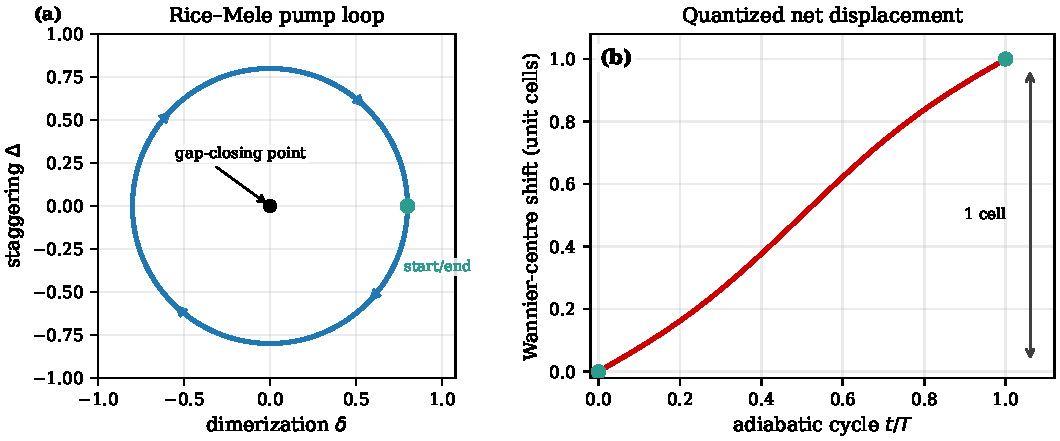
\includegraphics[width=0.95\textwidth]{figures/fig_ch14_ricemele_pump_step178.pdf}
  \caption{Rice--Mele topological pump.
  (a)~Counter-clockwise parameter loop in the $(\delta,\Delta)$-plane
  enclosing the gap-closing origin (black dot).  Blue arrows indicate the
  traversal direction; the teal dot marks the start/end point.
  (b)~Wannier-centre displacement (in unit cells) during one adiabatic cycle.
  The net shift of exactly one cell (double arrow) is the topological
  invariant of the pump; it equals the Chern number $\mathcal{C}=1$
  of the filled band over the parameter torus.}
  \label{fig:ch14-ricemele-pump}
\end{figure}

\subsection{Quantitative analysis of the photonic SSH edge mode}
\label{sec:ch14-ssh-quantitative}

For a finite SSH chain of $N$ unit cells terminated at a weak bond
(so the first coupling is $t_1<t_2$), the edge-mode wavefunction
at site $n$ on sublattice $A$ is
\begin{equation}\label{eq:ch14-ssh-edge-wfn}
  \psi_n^A = \mathcal{N}\left(-\frac{t_1}{t_2}\right)^n, \qquad
  \psi_n^B = 0\,,
\end{equation}
where $\mathcal{N}$ is a normalisation constant and the mode lives
entirely on sublattice $A$.  The sublattice polarisation of the edge
mode is a direct consequence of the chiral symmetry
$\Gamma H\Gamma=-H$ with $\Gamma=\sigma_z$: at mid-gap energy
$E=0$, the eigenstate can be chosen to have support on only one
sublattice.

The localisation length is
\begin{equation}\label{eq:ch14-ssh-loc-length}
  \xi = \frac{a}{\ln(t_2/t_1)}\,,
\end{equation}
where $a$ is the lattice constant.  As the gap closes
($t_1\to t_2$), the localisation length diverges and the edge mode
delocalises---a hallmark of the topological phase transition.

In a photonic waveguide array, the coupling constants depend
exponentially on the inter-waveguide separation $d$:
$t\approx t_0\exp(-d/d_0)$, where $d_0$ is a decay length set by
the evanescent tail of the waveguide mode (typically
$d_0\sim 1$--$3\;\mu\mathrm{m}$ in silica or silicon).  The
dimerisation ratio $t_1/t_2$ can therefore be tuned continuously by
adjusting the two gap widths, allowing systematic exploration of the
topological phase diagram \cite{ozawa2018topological}.

\begin{figure}[t]
  \centering
  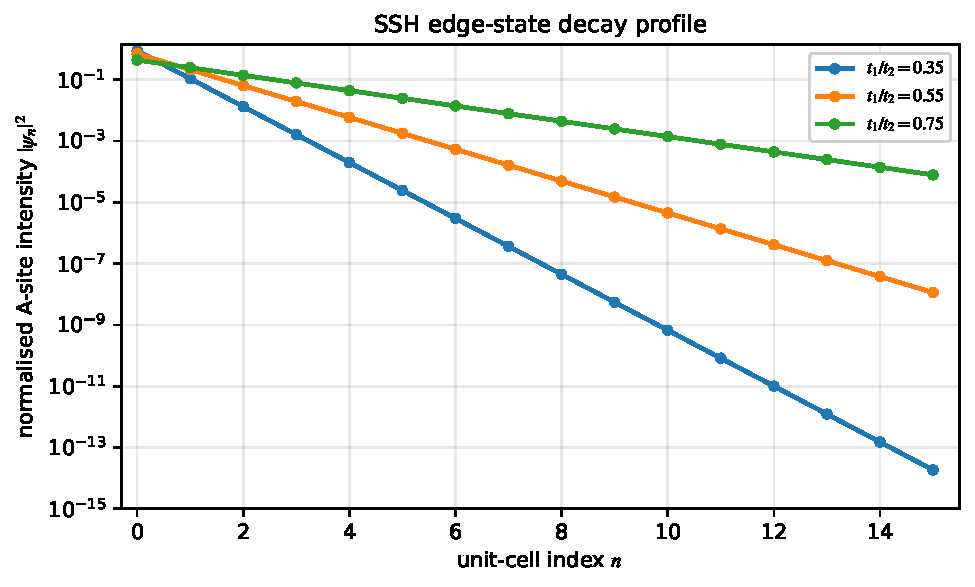
\includegraphics[width=0.78\textwidth]{figures/fig_ch14_ssh_edge_decay.pdf}
  \caption{SSH edge-state localisation.  For $t_1<t_2$, the edge-state
  intensity decays as $(t_1/t_2)^{2n}$ into the bulk.  As the dimerisation
  weakens and $t_1/t_2\to1$, the localisation length diverges at the
  topological phase transition.}
  \label{fig:ch14-ssh-edge-decay}
\end{figure}

\section{Beyond SSH: the Rice--Mele model}
\label{sec:ch14-rice-mele}

The SSH model has chiral symmetry $\sigma_z H \sigma_z = -H$, which
pins the edge-state energy to zero and quantises the Zak phase to $0$
or $\pi$.  Breaking chiral symmetry by adding a staggered on-site
potential $\Delta$ produces the Rice--Mele model
\cite{asbth2016berry,ozawa2018topological}:
\begin{equation}\label{eq:ch14-rice-mele}
  H_{\mathrm{RM}}(k) = \bigl(t_1 + t_2\cos ka\bigr)\sigma_x
  + t_2\sin(ka)\,\sigma_y + \Delta\,\sigma_z\,.
\end{equation}
The energy spectrum is
$E_\pm(k) = \pm\sqrt{(t_1+t_2\cos ka)^2 + t_2^2\sin^2(ka) + \Delta^2}$,
and a gap exists for all $\Delta\neq 0$ even when $t_1 = t_2$.

\subsection{Topology of the Rice--Mele model}
\label{sec:ch14-rm-topology}

Because chiral symmetry is broken, the winding number $\nu$ is no longer
well defined and the Zak phase is no longer quantised.  Instead, the
relevant topological invariant is the polarisation change
$\Delta P$ accumulated over one adiabatic cycle in the two-parameter
space $(\delta t, \Delta)$, where $\delta t = t_1 - t_2$.  If the
cycle encloses the gap-closing point $(\delta t, \Delta) = (0,0)$,
the polarisation change is quantised:
\begin{equation}\label{eq:ch14-rm-polarisation}
  \Delta P = \frac{e}{2\pi}\oint \mathcal{A}(k,\theta)\,\dd\theta
  = \pm e\,,
\end{equation}
where $\theta$ parametrises the cycle.  This is precisely the Thouless
pump of Section~\ref{sec:ch14-thouless}: the $(k,\theta)$ torus carries
a Chern number $\Chern = \pm 1$.

The Rice--Mele model therefore provides the minimal framework for
understanding how the interplay of dimerisation and inversion breaking
controls the topology of one-dimensional photonic systems.  In a
photonic implementation, $\Delta$ corresponds to a detuning between
the resonance frequencies of the two sublattice sites, which can be
introduced by varying the waveguide width or the resonator radius
\cite{ozawa2018topological,price2022roadmap}.

\subsection{Photonic Rice--Mele experiments}
\label{sec:ch14-rm-photonic}

Photonic Rice--Mele systems have been realised in coupled-waveguide
arrays where both the coupling constants and the propagation constants
are modulated along the propagation axis.  By slowly cycling the
modulation parameters through a closed loop that encloses the
degeneracy point, the quantised adiabatic pumping of light intensity
has been observed experimentally.

Cerjan et~al.\ (2020) demonstrated a photonic Rice--Mele pump in a
silicon photonic lattice, observing quantised displacement of light
over multiple pump cycles with high fidelity.  The deviation from
integer displacement was less than 3\%, limited primarily by
non-adiabatic corrections from the finite propagation length
\cite{price2022roadmap}.

\section{Bulk-boundary correspondence in one dimension}
\label{sec:ch14-bbc-1d}

The hallmark of topological phases is the bulk-boundary correspondence:
a nontrivial bulk invariant guarantees the existence of boundary-localised
states.  In one dimension, this correspondence takes a particularly
transparent form \cite{asbth2016berry}.

\subsection{The winding number predicts edge states}
\label{sec:ch14-winding-edge}

Consider a semi-infinite SSH chain occupying sites $n = 0, 1, 2, \ldots$
with the weak bond $t_1$ at the boundary.  The bulk winding number
$\nu$ (Section~\ref{sec:ch14-1d-invariants}) counts the number of
zero-energy edge states per boundary:
\begin{equation}\label{eq:ch14-bbc-winding}
  N_{\mathrm{edge}} = |\nu|\,.
\end{equation}
For $\nu = 1$ (the topological phase with $t_1 < t_2$), there is
exactly one edge state; for $\nu = 0$ (trivial phase), there are none.
This is a rigorous mathematical theorem, not merely an observation
from specific models: it follows from the index theory of Fredholm
operators acting on the half-line
\cite{asbth2016berry}.

\subsection{Robustness and symmetry protection}
\label{sec:ch14-robustness}

The topological protection of the SSH edge state requires chiral
(sublattice) symmetry.  Under arbitrary perturbations that preserve
chiral symmetry---such as random variations of the coupling
constants $t_1$ and $t_2$, or long-range hopping that respects the
sublattice structure---the edge state remains pinned at zero energy.

When chiral symmetry is broken (e.g.\ by adding random on-site
potentials), the edge-state energy shifts away from zero.  However,
the state itself does not disappear until the perturbation closes
the bulk gap.  The topological origin of the state manifests as an
anomalously long lifetime compared to generic disorder-induced states
\cite{ozawa2018topological}.

In photonic implementations, chiral symmetry corresponds to a
balance between the effective ``on-site energies'' of the two
sublattice waveguides.  Fabrication imperfections that change the
waveguide widths asymmetrically break this symmetry, while
imperfections that change both sublattice sites equally preserve it.
Careful waveguide design can therefore maximise topological protection
in realistic devices \cite{wu2015scheme,price2022roadmap}.

\subsection{Connection to higher dimensions}
\label{sec:ch14-higher-dim-connection}

One-dimensional topology is intimately connected to higher-dimensional
topological phases through dimensional reduction.  The Thouless pump
(Section~\ref{sec:ch14-thouless}) provides the clearest example: the
$(k, \theta)$ parameter space of a one-dimensional pump is
topologically equivalent to the Brillouin zone of a two-dimensional
quantum Hall system, and the pump's Chern number equals the Hall
conductance of the parent 2D system \cite{thouless1982quantized}.

This dimensional hierarchy extends further.  A two-parameter family of
one-dimensional systems, with parameters $(\theta_1, \theta_2)$, can
realise a second Chern number---a four-dimensional topological
invariant.  Zilberberg et~al.\ (2018) exploited this correspondence
to observe signatures of four-dimensional quantum Hall physics in a
two-dimensional photonic waveguide array, where the two spatial
dimensions encoded the physical coordinate and one pump parameter,
while the second pump parameter was scanned experimentally
\cite{price2022roadmap,ozawa2018topological}.

The lesson is that one-dimensional photonic systems, despite their
apparent simplicity, serve as building blocks for exploring topological
physics in arbitrary dimensions.  The synthetic-dimension approach of
Chapter~\ref{ch:synthetic-dimensions} generalises this idea by
promoting internal degrees of freedom (frequency, orbital angular
momentum, or spin) to additional lattice dimensions
\cite{kim2020recent,guglielmon2017photonic}.

\section*{Exercises}

\begin{exercise}
  Show that the winding number \eqref{eq:ch14-winding} of the SSH model
  changes from 0 to 1 at $J_1=J_2$, where the band gap closes.
  Sketch the trajectory of $(d_x(k),d_y(k))$ for $J_1>J_2$, $J_1=J_2$,
  and $J_1<J_2$.
\end{exercise}

\begin{exercise}
  For the coupled-cavity SSH chain with $\omega_0$, $J_1$, $J_2$, show
  that the interface mode has frequency $\omega=\omega_0$ (mid-gap) and
  verify the exponential localisation \eqref{eq:ch14-interface-mode}.
\end{exercise}

\begin{exercise}
  Derive the band structure of a 1D Bragg stack from the transfer
  matrix \eqref{eq:ch14-transfer-matrix} and the Bloch condition
  \eqref{eq:ch14-bloch-condition}.  Show that a gap opens when
  $n_Ad_A\neq n_Bd_B$.  Compute the Zak phase for the lowest band
  when $n_Ad_A>n_Bd_B$ and when $n_Ad_A<n_Bd_B$.
\end{exercise}

\begin{exercise}
  Verify equation \eqref{eq:ch14-localisation-length} by computing the
  envelope of the interface mode \eqref{eq:ch14-interface-mode} and
  extracting the $1/\ee$ decay length.
\end{exercise}

\begin{exercise}
  Design a Thouless pump for a 1D photonic crystal by specifying a
  two-parameter family of unit cells such that the Chern number in
  $(k,\theta)$ space is nonzero.  \emph{Hint:} use the Rice--Mele
  model (SSH with an added staggered on-site potential that varies
  with $\theta$).
\end{exercise}

\begin{exercise}
  Show that chiral symmetry ($\sigma_z H\sigma_z=-H$) forces the
  interface mode of the SSH model to have exactly zero energy.  What
  happens to the interface mode frequency when chiral symmetry is
  broken by adding a staggered potential $\Delta\sigma_z$?
\end{exercise}
